\begin{figure}[h!]
	\centering
	
	
	\tikzset{every picture/.style={line width=0.75pt}} %set default line width to 0.75pt        
	
	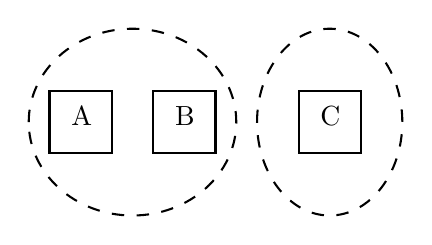
\begin{tikzpicture}[x=0.75pt,y=0.75pt,yscale=-1,xscale=1]
		%uncomment if require: \path (0,300); %set diagram left start at 0, and has height of 300
		
		%Shape: Square [id:dp45846669475066437] 
		\draw   (180,80) -- (210,80) -- (210,110) -- (180,110) -- cycle ;
		%Shape: Square [id:dp8694832240743474] 
		\draw   (230,80) -- (260,80) -- (260,110) -- (230,110) -- cycle ;
		%Shape: Square [id:dp9643149276555201] 
		\draw   (300,80) -- (330,80) -- (330,110) -- (300,110) -- cycle ;
		%Shape: Ellipse [id:dp7472268647554123] 
		\draw  [dash pattern={on 4.5pt off 4.5pt}] (170,95) .. controls (170,70.15) and (192.39,50) .. (220,50) .. controls (247.61,50) and (270,70.15) .. (270,95) .. controls (270,119.85) and (247.61,140) .. (220,140) .. controls (192.39,140) and (170,119.85) .. (170,95) -- cycle ;
		%Shape: Ellipse [id:dp9372300796607134] 
		\draw  [dash pattern={on 4.5pt off 4.5pt}] (280,95) .. controls (280,70.15) and (295.67,50) .. (315,50) .. controls (334.33,50) and (350,70.15) .. (350,95) .. controls (350,119.85) and (334.33,140) .. (315,140) .. controls (295.67,140) and (280,119.85) .. (280,95) -- cycle ;
		
		% Text Node
		\draw (189,86) node [anchor=north west][inner sep=0.75pt]   [align=left] {A};
		% Text Node
		\draw (239,86) node [anchor=north west][inner sep=0.75pt]   [align=left] {B};
		% Text Node
		\draw (309,86) node [anchor=north west][inner sep=0.75pt]   [align=left] {C};
		
		
	\end{tikzpicture}
\end{figure}